\documentclass[a4paper, twoside, english]{article}

\usepackage{amsmath}
\usepackage{amsfonts}
\usepackage{ihci}
\usepackage{graphicx}
\usepackage{subfig}

\graphicspath{{./../figures/}}
\newcommand{\br}{\textbf{R}}
\newcommand{\qed}{\hfill \ensuremath{\Box}}


\title{Exercise 1 \\ 3D Computer Vision}  % Replace "Template Report" with Exercise 1, Exercise 2, etc
\author{Jingyuan Sha}                       % Replace with your names
\date{12.11.2021}                              % Replace with current date

\begin{document}

\maketitle

\part{Theory}

\section{Properties of Rotation Matrices}

\begin{enumerate}
	\item Let   $ \br_{i\cdot}, \br_{\cdot j}$ denote i-th row and j-th column of $ \br $ separately, where $ i\neq j $. 
	
	$ \br $ is orthogonal matrix \\
	$\Rightarrow$ $ \br \cdot \br^T =  \textbf{I} $\\
	$ \Rightarrow \br_{i\cdot} \cdot \br_{\cdot j}^T = 0, (i\neq j) $\\
	$ \Rightarrow \br_{i\cdot}, \br_{\cdot j}^T $ are orthogonal\\
	since $ \br_{\cdot j}^T = \br_{j \cdot} $,\\
	therefore, $ \br_{i\cdot} \cdot \br_{j \cdot} = 0, (i\neq j) $ (rows orthogonal)\\
	same, based on $ \br^T \cdot \br =  \textbf{I} $ we have columns orthogonal.\\
	
	$ \br \cdot \br^T = \textbf{I} $\\
	$ \Rightarrow \br_{i\cdot} \cdot \br_{\cdot i}^T = 1$\\
	since $ \br_{\cdot i}^T = \br_{i\cdot} $, \\
	thus $ \br_{i\cdot} \cdot \br_{i\cdot} = 1  $\\
	$ \Rightarrow \| \br_{i\cdot}  \| = 1 $ $ \Rightarrow $ each row of $ \br $ has length $ 1 $.\\
	same, based on  $ \br^T \cdot \br =  \textbf{I} $ we can prove each column of $ \br $ has length $ 1 $. \qed
	
	\item
	
	\begin{itemize}
		\item Rotation matrix by $ \psi $ around $ z $ axis is
		\begin{equation*}
			\br_z(\psi) = \left[
			\begin{array}{ccc}
				\cos \psi & -\sin \psi & 0 \\
				\sin \psi & \cos \psi & 0 \\
				0 & 0 & 1
			\end{array}
			\right],
		\end{equation*}
		the inverse is
		\begin{equation*}
			\br_z^{-1}(\psi) = \left[
			\begin{array}{ccc}
				\cos \psi & \sin \psi & 0 \\
				-\sin \psi & \cos \psi & 0 \\
				0 & 0 & 1
			\end{array}
			\right] = \br_z^T(\psi),
		\end{equation*}
		
		And also, 
		\begin{equation*}
			\det(\br_z) = \cos \psi \cdot \cos \psi -\sin \psi \cdot (-\sin \psi) + 0 = 1
		\end{equation*}
		Thus $ \br_z(\psi) $ fulfills the properties of rotation matrices for any angles $ \psi $.
		
		\item 
		
		Rotation matrix by $ \theta $ around $ y $ axis is
		\begin{equation*}
			\br_y(\theta) = \left[
			\begin{array}{ccc}
				\cos \theta & 0 & \sin \theta \\
				0 & 1 & 0 \\
				-\sin \theta & 0 & \cos \theta
			\end{array}
			\right],
		\end{equation*}
		the inverse is
		\begin{equation*}
			\br_y^T(\theta) = \left[
			\begin{array}{ccc}
				\cos \theta & 0 & -\sin \theta \\
				0 & 1 & 0 \\
				\sin \theta & 0 & \cos \theta
			\end{array}
			\right]= \br_y^{-1}(\theta),
		\end{equation*}	
		
		And also, 
		\begin{equation*}
			\det(\br_y) = \cos \theta \cdot \cos \theta + 0 + \sin \theta \cdot (0-(-\sin \theta)) = 1
		\end{equation*}
		Thus $ \br_y(\theta) $ fulfills the properties of rotation matrices for any angles $ \theta $.
		
		
		\item 
		
		Rotation matrix by $ \phi $ around $ x $ axis is
		\begin{equation*}
			\br_x(\phi) = \left[
			\begin{array}{ccc}
				1 & 0 & 0 \\
				0 & \cos \phi & -\sin \phi \\
				0 & \sin \phi & \cos \phi
			\end{array}
			\right],
		\end{equation*}
		the inverse is
		\begin{equation*}
			\br_x(\phi) = \left[
			\begin{array}{ccc}
				1 & 0 & 0 \\
				0 & \cos \phi & \sin \phi \\
				0 & -\sin \phi & \cos \phi
			\end{array}
			\right] = \br_x^{-1}(\phi),
		\end{equation*}
		
		And also, 
		\begin{equation*}
			\det(\br_x) = \cos \phi \cdot \cos \phi - (-\sin \phi)\cdot \sin \phi + 0 + 0 = 1
		\end{equation*}
		Thus $ \br_x(\phi) $ fulfills the properties of rotation matrices for any angles $ \phi $.
		
		\item 
		Since 
		\begin{equation*}
			\br = \br_z(\psi) \br_y(\theta) \br_x(\phi) \\
		\end{equation*}
		Thus, 
		\begin{equation*}
			\begin{aligned}
				\br^{-1} 
				&= (\br_z(\psi) \br_y(\theta) \br_x(\phi))^{-1}\\
				&= \br_x^{-1}\br_y^{-1}\br_z^{-1}\\
				&=\br_x^T \br_y^T \br_z^T\\
				&=(\br_z \br_y \br_x)^T\\
				&=\br^T
			\end{aligned}
		\end{equation*}
		
		\begin{equation*}
			\det (\br) = \det (\br_z \br_y \br_x) = \det (\br_z) \det (\br_y) \det (\br_x) = 1\cdot 1 \cdot 1 = 1
		\end{equation*}	\qed	

	\end{itemize} 	
	
	\item 
	The geometric interpretation of the determinant of a square $ 3\times 3 $ matrix is the scale of the matrix. Rotation matrix have to have determinant 1, because the rotation operation is performed by multiple original object with rotation matrix, which should not change the scale of the object, thus it has to be with determinant 1.
	
	 
\end{enumerate}

\section{Transformation Chain}
The transformation chain is 
	\[ \text{World coordinate } \left(
	\begin{array}{c}
		X_s \\
		Y_s \\
		Z_s\\
	\end{array}
	\right) 
	\rightarrow \text{Camera coordinate} 
	\left(
	\begin{array}{c}
		x_s \\
		y_s \\
		z_s\\
	\end{array}
	\right)
	\rightarrow 
		\text{pixel coordinate}
		\left(
		\begin{array}{c}
			x_{pix} \\
			y_{pix} 
		\end{array}
		\right)
	\]

\begin{equation*}
	\left(
	\begin{array}{c}
		u\prime \\
		v\prime \\
		w\prime
	\end{array}
	\right) = K(I_3 | 0_3)
	\left(
	\begin{array}{c}
		x_s \\
		y_s \\
		z_s\\
		1
	\end{array}
	\right)
	,
\end{equation*}
where

\begin{equation*}
	\left(
	\begin{array}{c}
		x_s \\
		y_s \\
		z_s\\
	\end{array}
	\right) = 
	\left(
	\begin{array}{c}
		t_x \\
		t_y \\
		t_z\\
	\end{array}
	\right) + \br 
	\left(
	\begin{array}{c}
		X_s \\
		Y_s \\
		Z_s\\
	\end{array}
	\right)
\end{equation*}
Pixel coordinate
\begin{equation*}
	\begin{cases}
		x_{pix} = \frac{u\prime}{w\prime}\\
		y_{pix} = \frac{v\prime}{w\prime}
	\end{cases}
\end{equation*}

\newpage

\part{Implementation}


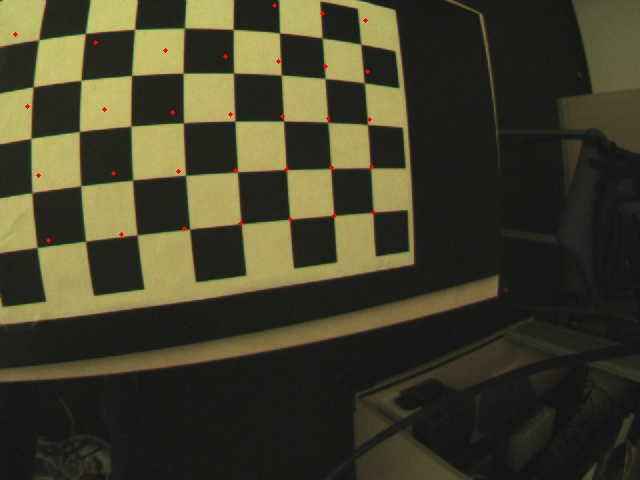
\includegraphics[width=0.8\textwidth]{red_0.jpg} \\
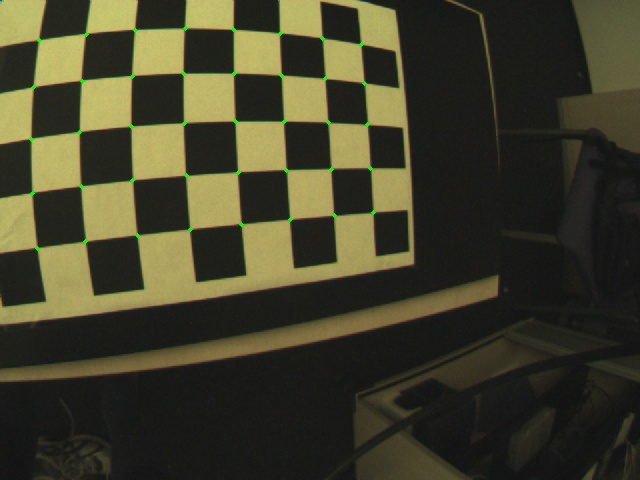
\includegraphics[width=0.8\textwidth]{green_0.jpg}


\end{document}